


\begin{figure}
    \centering
    \begin{subfigure}[tb]{0.48\textwidth}
        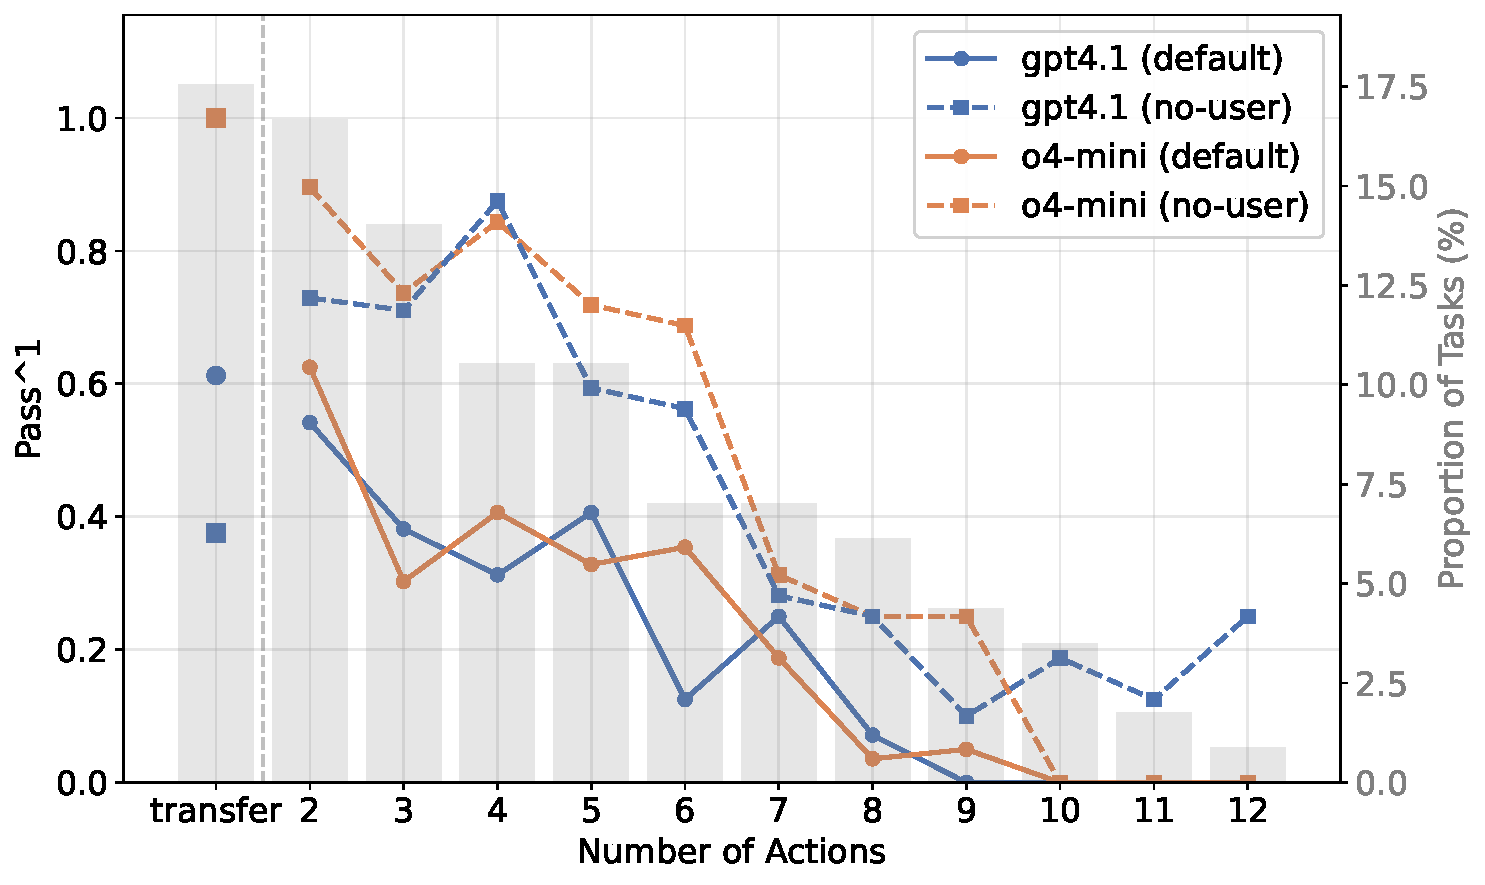
\includegraphics[width=\textwidth]{figures/results/pass_k_vs_num_actions_telecom_all_modes_llm_comparison.pdf}
    \end{subfigure}
    \hfill
    \begin{subfigure}[tb]{0.48\textwidth}
        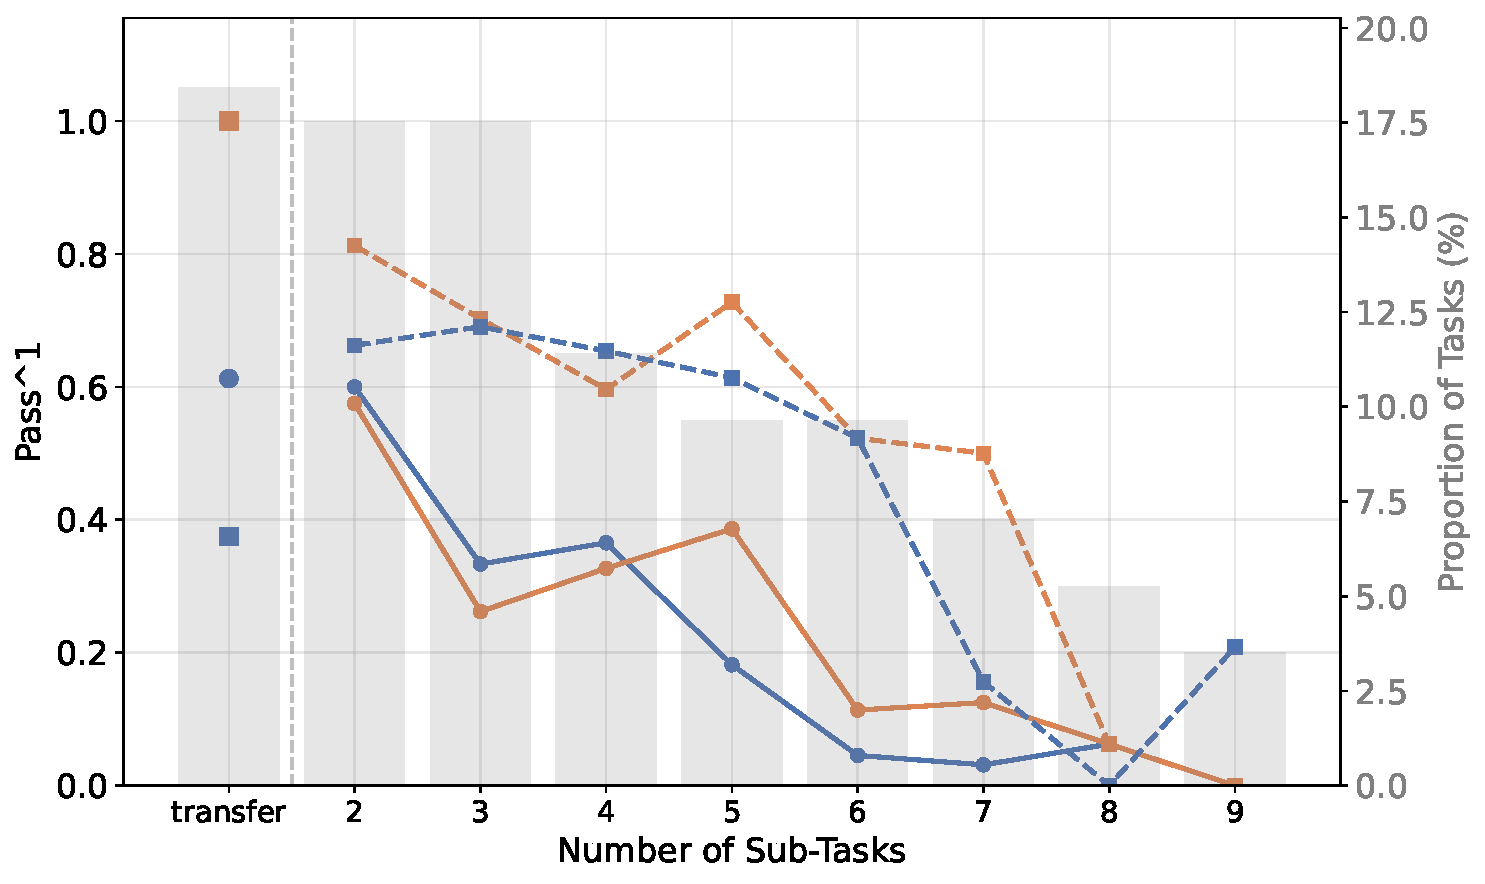
\includegraphics[width=\textwidth]{figures/results/pass_k_vs_num_issues_telecom_all_modes_llm_comparison.pdf}
    \end{subfigure}
    \vspace{-0.5em}
    \caption{\telecom의 다양한 과제에 대한 \passone 점수. 해결에 필요한 행동 수(왼쪽) 또는 처리해야 할 서로 다른 문제 수(오른쪽)에 따라 구간화했다. \textit{transfer}는 사람에게 이관해야 하며 에이전트 단독으로는 해결할 수 없는 과제의 특수한 경우를 가리킨다. (회색 막대는 해당 구간에 속하는 과제의 비율을 나타낸다.)}
    \label{fig:telecom_results}
\end{figure}


